\documentclass[a4paper,twoside,11pt]{article}

\usepackage[utf8]{inputenc}
\usepackage[OT1]{fontenc}
\usepackage[czech]{babel}
\usepackage{graphicx}
\usepackage[margin=2cm]{geometry}

\title{Provozní záznamy JE Třeskoprsky}
\author{Informatika pro moderní fyziky (5)}

\begin{document}

\maketitle

\tableofcontents

\section{Grafy}

\subsection{Koncentrace kyseliny borité}



\subsubsection{Kampaň c01}

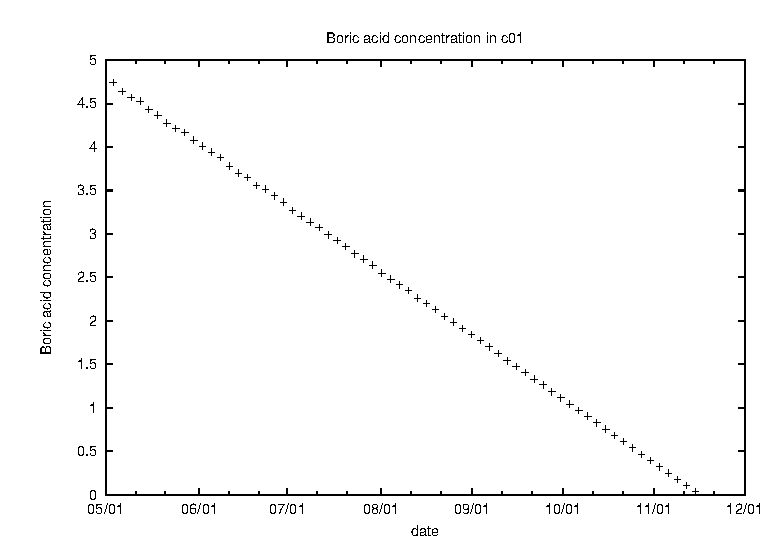
\includegraphics[width=0.8\textwidth]{data_c01_bc.eps}


\subsubsection{Kampaň c02}

\includegraphics[width=0.8\textwidth]{data_c02_bc.eps}


\subsubsection{Kampaň c03}

\includegraphics[width=0.8\textwidth]{data_c03_bc.eps}


\subsubsection{Kampaň c04}

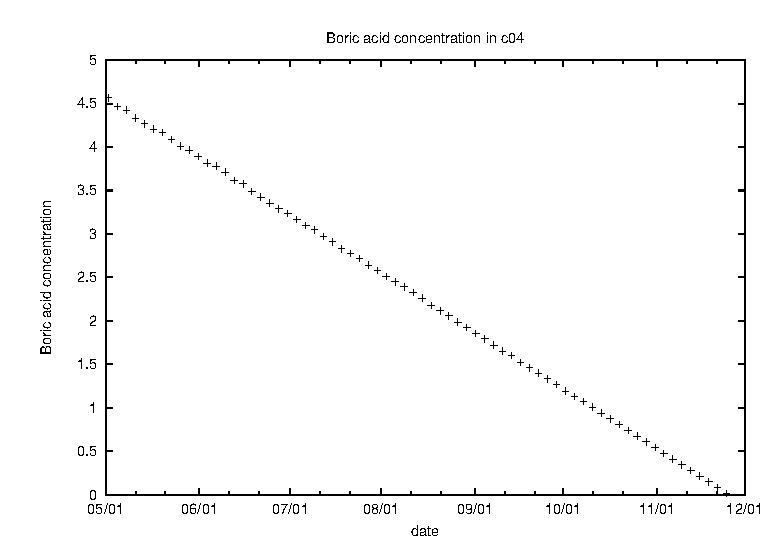
\includegraphics[width=0.8\textwidth]{data_c04_bc.eps}


\subsubsection{Kampaň c05}

\includegraphics[width=0.8\textwidth]{data_c05_bc.eps}


\subsection{Axiální ofset}



\subsubsection{Kampaň c01}

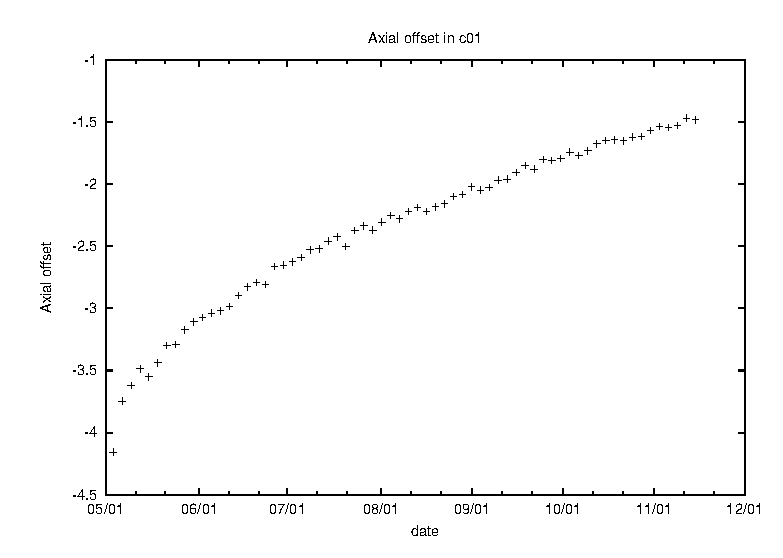
\includegraphics[width=0.8\textwidth]{data_c01_ao.eps}


\subsubsection{Kampaň c02}

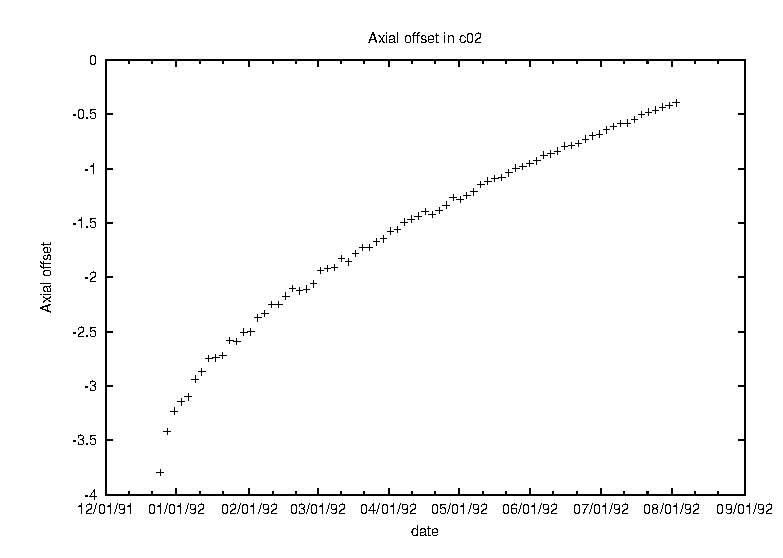
\includegraphics[width=0.8\textwidth]{data_c02_ao.eps}


\subsubsection{Kampaň c03}

\includegraphics[width=0.8\textwidth]{data_c03_ao.eps}


\subsubsection{Kampaň c04}

\includegraphics[width=0.8\textwidth]{data_c04_ao.eps}


\subsubsection{Kampaň c05}

\includegraphics[width=0.8\textwidth]{data_c05_ao.eps}


\section{Tabulky}

\subsection{Koncentrace kyseliny borité}



\subsubsection{Kampaň c01}

\begin{tabular}{|l|l||l|l||l|l|}
\hline
Datum & cB [g/kg] & Datum & cB [g/kg] & Datum & cB [g/kg] \\
\hline
05/04/1991 & 4.741 & 
05/07/1991 & 4.637 & 
05/10/1991 & 4.571 \\
\hline
05/13/1991 & 4.529 & 
05/16/1991 & 4.431 & 
05/19/1991 & 4.367 \\
\hline
05/22/1991 & 4.276 & 
05/25/1991 & 4.212 & 
05/28/1991 & 4.165 \\
\hline
05/31/1991 & 4.080 & 
06/03/1991 & 4.009 & 
06/06/1991 & 3.942 \\
\hline
06/09/1991 & 3.877 & 
06/12/1991 & 3.779 & 
06/15/1991 & 3.701 \\
\hline
06/18/1991 & 3.651 & 
06/21/1991 & 3.556 & 
06/24/1991 & 3.514 \\
\hline
06/27/1991 & 3.438 & 
06/30/1991 & 3.365 & 
07/03/1991 & 3.272 \\
\hline
07/06/1991 & 3.203 & 
07/09/1991 & 3.134 & 
07/12/1991 & 3.073 \\
\hline
07/15/1991 & 2.989 & 
07/18/1991 & 2.923 & 
07/21/1991 & 2.856 \\
\hline
07/24/1991 & 2.770 & 
07/27/1991 & 2.708 & 
07/30/1991 & 2.641 \\
\hline
08/02/1991 & 2.550 & 
08/05/1991 & 2.479 & 
08/08/1991 & 2.412 \\
\hline
08/11/1991 & 2.346 & 
08/14/1991 & 2.261 & 
08/17/1991 & 2.202 \\
\hline
08/20/1991 & 2.131 & 
08/23/1991 & 2.051 & 
08/26/1991 & 1.983 \\
\hline
08/29/1991 & 1.914 & 
09/01/1991 & 1.842 & 
09/04/1991 & 1.773 \\
\hline
09/07/1991 & 1.700 & 
09/10/1991 & 1.623 & 
09/13/1991 & 1.540 \\
\hline
09/16/1991 & 1.475 & 
09/19/1991 & 1.405 & 
09/22/1991 & 1.328 \\
\hline
09/25/1991 & 1.263 & 
09/28/1991 & 1.182 & 
10/01/1991 & 1.113 \\
\hline
10/04/1991 & 1.040 & 
10/07/1991 & 0.968 & 
10/10/1991 & 0.902 \\
\hline
10/13/1991 & 0.827 & 
10/16/1991 & 0.754 & 
10/19/1991 & 0.683 \\
\hline
10/22/1991 & 0.610 & 
10/25/1991 & 0.538 & 
10/28/1991 & 0.463 \\
\hline
10/31/1991 & 0.393 & 
11/03/1991 & 0.319 & 
11/06/1991 & 0.249 \\
\hline
11/09/1991 & 0.175 & 
11/12/1991 & 0.104 & 
11/15/1991 & 0.032 \\
\hline

\end{tabular}



\subsubsection{Kampaň c02}

\begin{tabular}{|l|l||l|l||l|l|}
\hline
Datum & cB [g/kg] & Datum & cB [g/kg] & Datum & cB [g/kg] \\
\hline
12/25/1991 & 4.264 & 
12/28/1991 & 4.208 & 
12/31/1991 & 4.165 \\
\hline
01/03/1992 & 4.128 & 
01/06/1992 & 4.033 & 
01/09/1992 & 3.992 \\
\hline
01/12/1992 & 3.935 & 
01/15/1992 & 3.872 & 
01/18/1992 & 3.821 \\
\hline
01/21/1992 & 3.786 & 
01/24/1992 & 3.703 & 
01/27/1992 & 3.645 \\
\hline
01/30/1992 & 3.605 & 
02/02/1992 & 3.552 & 
02/05/1992 & 3.476 \\
\hline
02/08/1992 & 3.432 & 
02/11/1992 & 3.367 & 
02/14/1992 & 3.292 \\
\hline
02/17/1992 & 3.247 & 
02/20/1992 & 3.185 & 
02/23/1992 & 3.128 \\
\hline
02/26/1992 & 3.074 & 
02/29/1992 & 3.035 & 
03/03/1992 & 2.973 \\
\hline
03/06/1992 & 2.898 & 
03/09/1992 & 2.850 & 
03/12/1992 & 2.779 \\
\hline
03/15/1992 & 2.734 & 
03/18/1992 & 2.681 & 
03/21/1992 & 2.619 \\
\hline
03/24/1992 & 2.568 & 
03/27/1992 & 2.496 & 
03/30/1992 & 2.455 \\
\hline
04/02/1992 & 2.381 & 
04/05/1992 & 2.336 & 
04/08/1992 & 2.286 \\
\hline
04/11/1992 & 2.227 & 
04/14/1992 & 2.153 & 
04/17/1992 & 2.114 \\
\hline
04/20/1992 & 2.051 & 
04/23/1992 & 1.998 & 
04/26/1992 & 1.930 \\
\hline
04/29/1992 & 1.879 & 
05/02/1992 & 1.814 & 
05/05/1992 & 1.766 \\
\hline
05/08/1992 & 1.702 & 
05/11/1992 & 1.652 & 
05/14/1992 & 1.594 \\
\hline
05/17/1992 & 1.538 & 
05/20/1992 & 1.468 & 
05/23/1992 & 1.419 \\
\hline
05/26/1992 & 1.358 & 
05/29/1992 & 1.296 & 
06/01/1992 & 1.239 \\
\hline
06/04/1992 & 1.193 & 
06/07/1992 & 1.136 & 
06/10/1992 & 1.069 \\
\hline
06/13/1992 & 1.015 & 
06/16/1992 & 0.955 & 
06/19/1992 & 0.902 \\
\hline
06/22/1992 & 0.843 & 
06/25/1992 & 0.787 & 
06/28/1992 & 0.731 \\
\hline
07/01/1992 & 0.670 & 
07/04/1992 & 0.612 & 
07/07/1992 & 0.555 \\
\hline
07/10/1992 & 0.499 & 
07/13/1992 & 0.441 & 
07/16/1992 & 0.385 \\
\hline
07/19/1992 & 0.327 & 
07/22/1992 & 0.271 & 
07/25/1992 & 0.213 \\
\hline
07/28/1992 & 0.157 & 
07/31/1992 & 0.099 & 
08/03/1992 & 0.041 \\
\hline

\end{tabular}



\subsubsection{Kampaň c03}

\begin{tabular}{|l|l||l|l||l|l|}
\hline
Datum & cB [g/kg] & Datum & cB [g/kg] & Datum & cB [g/kg] \\
\hline
09/07/1992 & 4.415 & 
09/10/1992 & 4.354 & 
09/13/1992 & 4.295 \\
\hline
09/16/1992 & 4.233 & 
09/19/1992 & 4.149 & 
09/22/1992 & 4.079 \\
\hline
09/25/1992 & 3.999 & 
09/28/1992 & 3.938 & 
10/01/1992 & 3.879 \\
\hline
10/04/1992 & 3.822 & 
10/07/1992 & 3.741 & 
10/10/1992 & 3.663 \\
\hline
10/13/1992 & 3.613 & 
10/16/1992 & 3.545 & 
10/19/1992 & 3.485 \\
\hline
10/22/1992 & 3.409 & 
10/25/1992 & 3.336 & 
10/28/1992 & 3.273 \\
\hline
10/31/1992 & 3.214 & 
11/03/1992 & 3.139 & 
11/06/1992 & 3.058 \\
\hline
11/09/1992 & 3.004 & 
11/12/1992 & 2.940 & 
11/15/1992 & 2.881 \\
\hline
11/18/1992 & 2.806 & 
11/21/1992 & 2.749 & 
11/24/1992 & 2.659 \\
\hline
11/27/1992 & 2.602 & 
11/30/1992 & 2.541 & 
12/03/1992 & 2.479 \\
\hline
12/06/1992 & 2.394 & 
12/09/1992 & 2.340 & 
12/12/1992 & 2.262 \\
\hline
12/15/1992 & 2.205 & 
12/18/1992 & 2.141 & 
12/21/1992 & 2.063 \\
\hline
12/24/1992 & 1.998 & 
12/27/1992 & 1.940 & 
12/30/1992 & 1.858 \\
\hline
01/02/1993 & 1.799 & 
01/05/1993 & 1.723 & 
01/08/1993 & 1.663 \\
\hline
01/11/1993 & 1.604 & 
01/14/1993 & 1.527 & 
01/17/1993 & 1.460 \\
\hline
01/20/1993 & 1.389 & 
01/23/1993 & 1.329 & 
01/26/1993 & 1.266 \\
\hline
01/29/1993 & 1.195 & 
02/01/1993 & 1.129 & 
02/04/1993 & 1.054 \\
\hline
02/07/1993 & 0.996 & 
02/10/1993 & 0.922 & 
02/13/1993 & 0.860 \\
\hline
02/16/1993 & 0.793 & 
02/19/1993 & 0.725 & 
02/22/1993 & 0.655 \\
\hline
02/25/1993 & 0.591 & 
02/28/1993 & 0.521 & 
03/03/1993 & 0.456 \\
\hline
03/06/1993 & 0.388 & 
03/09/1993 & 0.320 & 
03/12/1993 & 0.253 \\
\hline
03/15/1993 & 0.188 & 
03/18/1993 & 0.120 & 
03/21/1993 & 0.053 \\
\hline

\end{tabular}



\subsubsection{Kampaň c04}

\begin{tabular}{|l|l||l|l||l|l|}
\hline
Datum & cB [g/kg] & Datum & cB [g/kg] & Datum & cB [g/kg] \\
\hline
05/02/1993 & 4.566 & 
05/05/1993 & 4.465 & 
05/08/1993 & 4.423 \\
\hline
05/11/1993 & 4.332 & 
05/14/1993 & 4.266 & 
05/17/1993 & 4.207 \\
\hline
05/20/1993 & 4.166 & 
05/23/1993 & 4.087 & 
05/26/1993 & 4.011 \\
\hline
05/29/1993 & 3.963 & 
06/01/1993 & 3.892 & 
06/04/1993 & 3.814 \\
\hline
06/07/1993 & 3.779 & 
06/10/1993 & 3.711 & 
06/13/1993 & 3.617 \\
\hline
06/16/1993 & 3.575 & 
06/19/1993 & 3.486 & 
06/22/1993 & 3.422 \\
\hline
06/25/1993 & 3.356 & 
06/28/1993 & 3.289 & 
07/01/1993 & 3.236 \\
\hline
07/04/1993 & 3.166 & 
07/07/1993 & 3.094 & 
07/10/1993 & 3.047 \\
\hline
07/13/1993 & 2.972 & 
07/16/1993 & 2.908 & 
07/19/1993 & 2.829 \\
\hline
07/22/1993 & 2.774 & 
07/25/1993 & 2.717 & 
07/28/1993 & 2.641 \\
\hline
07/31/1993 & 2.582 & 
08/03/1993 & 2.512 & 
08/06/1993 & 2.448 \\
\hline
08/09/1993 & 2.392 & 
08/12/1993 & 2.327 & 
08/15/1993 & 2.260 \\
\hline
08/18/1993 & 2.179 & 
08/21/1993 & 2.114 & 
08/24/1993 & 2.056 \\
\hline
08/27/1993 & 1.983 & 
08/30/1993 & 1.921 & 
09/02/1993 & 1.855 \\
\hline
09/05/1993 & 1.792 & 
09/08/1993 & 1.720 & 
09/11/1993 & 1.651 \\
\hline
09/14/1993 & 1.600 & 
09/17/1993 & 1.521 & 
09/20/1993 & 1.458 \\
\hline
09/23/1993 & 1.397 & 
09/26/1993 & 1.334 & 
09/29/1993 & 1.266 \\
\hline
10/02/1993 & 1.193 & 
10/05/1993 & 1.130 & 
10/08/1993 & 1.072 \\
\hline
10/11/1993 & 1.006 & 
10/14/1993 & 0.937 & 
10/17/1993 & 0.871 \\
\hline
10/20/1993 & 0.807 & 
10/23/1993 & 0.736 & 
10/26/1993 & 0.673 \\
\hline
10/29/1993 & 0.607 & 
11/01/1993 & 0.542 & 
11/04/1993 & 0.475 \\
\hline
11/07/1993 & 0.408 & 
11/10/1993 & 0.343 & 
11/13/1993 & 0.279 \\
\hline
11/16/1993 & 0.213 & 
11/19/1993 & 0.147 & 
11/22/1993 & 0.082 \\
\hline

\end{tabular}



\subsubsection{Kampaň c05}

\begin{tabular}{|l|l||l|l||l|l|}
\hline
Datum & cB [g/kg] & Datum & cB [g/kg] & Datum & cB [g/kg] \\
\hline
01/03/1994 & 4.546 & 
01/06/1994 & 4.490 & 
01/09/1994 & 4.430 \\
\hline
01/12/1994 & 4.361 & 
01/15/1994 & 4.297 & 
01/18/1994 & 4.222 \\
\hline
01/21/1994 & 4.157 & 
01/24/1994 & 4.078 & 
01/27/1994 & 4.006 \\
\hline
01/30/1994 & 3.922 & 
02/02/1994 & 3.866 & 
02/05/1994 & 3.788 \\
\hline
02/08/1994 & 3.721 & 
02/11/1994 & 3.680 & 
02/14/1994 & 3.606 \\
\hline
02/17/1994 & 3.524 & 
02/20/1994 & 3.461 & 
02/23/1994 & 3.375 \\
\hline
02/26/1994 & 3.318 & 
03/01/1994 & 3.238 & 
03/04/1994 & 3.190 \\
\hline
03/07/1994 & 3.108 & 
03/10/1994 & 3.032 & 
03/13/1994 & 2.983 \\
\hline
03/16/1994 & 2.904 & 
03/19/1994 & 2.832 & 
03/22/1994 & 2.773 \\
\hline
03/25/1994 & 2.699 & 
03/28/1994 & 2.621 & 
03/31/1994 & 2.550 \\
\hline
04/03/1994 & 2.481 & 
04/06/1994 & 2.418 & 
04/09/1994 & 2.347 \\
\hline
04/12/1994 & 2.281 & 
04/15/1994 & 2.218 & 
04/18/1994 & 2.136 \\
\hline
04/21/1994 & 2.062 & 
04/24/1994 & 1.993 & 
04/27/1994 & 1.925 \\
\hline
04/30/1994 & 1.863 & 
05/03/1994 & 1.786 & 
05/06/1994 & 1.727 \\
\hline
05/09/1994 & 1.662 & 
05/12/1994 & 1.584 & 
05/15/1994 & 1.517 \\
\hline
05/18/1994 & 1.444 & 
05/21/1994 & 1.379 & 
05/24/1994 & 1.306 \\
\hline
05/27/1994 & 1.239 & 
05/30/1994 & 1.177 & 
06/02/1994 & 1.108 \\
\hline
06/05/1994 & 1.037 & 
06/08/1994 & 0.960 & 
06/11/1994 & 0.899 \\
\hline
06/14/1994 & 0.825 & 
06/17/1994 & 0.757 & 
06/20/1994 & 0.691 \\
\hline
06/23/1994 & 0.618 & 
06/26/1994 & 0.552 & 
06/29/1994 & 0.478 \\
\hline
07/02/1994 & 0.411 & 
07/05/1994 & 0.342 & 
07/08/1994 & 0.274 \\
\hline
07/11/1994 & 0.203 & 
07/14/1994 & 0.134 & 
07/17/1994 & 0.065 \\
\hline

\end{tabular}



\subsection{Axiální ofset}



\subsubsection{Kampaň c01}

\begin{tabular}{|l|l||l|l||l|l|}
\hline
Datum & ofset [\%] & Datum & ofset [\%] & Datum & ofset [\%]\\
\hline
05/04/1991 & -4.158 & 
05/07/1991 & -3.747 & 
05/10/1991 & -3.622 \\
\hline
05/13/1991 & -3.486 & 
05/16/1991 & -3.551 & 
05/19/1991 & -3.439 \\
\hline
05/22/1991 & -3.297 & 
05/25/1991 & -3.290 & 
05/28/1991 & -3.174 \\
\hline
05/31/1991 & -3.109 & 
06/03/1991 & -3.075 & 
06/06/1991 & -3.039 \\
\hline
06/09/1991 & -3.020 & 
06/12/1991 & -2.986 & 
06/15/1991 & -2.897 \\
\hline
06/18/1991 & -2.826 & 
06/21/1991 & -2.791 & 
06/24/1991 & -2.807 \\
\hline
06/27/1991 & -2.661 & 
06/30/1991 & -2.651 & 
07/03/1991 & -2.625 \\
\hline
07/06/1991 & -2.591 & 
07/09/1991 & -2.528 & 
07/12/1991 & -2.520 \\
\hline
07/15/1991 & -2.459 & 
07/18/1991 & -2.423 & 
07/21/1991 & -2.500 \\
\hline
07/24/1991 & -2.372 & 
07/27/1991 & -2.335 & 
07/30/1991 & -2.370 \\
\hline
08/02/1991 & -2.306 & 
08/05/1991 & -2.252 & 
08/08/1991 & -2.279 \\
\hline
08/11/1991 & -2.218 & 
08/14/1991 & -2.187 & 
08/17/1991 & -2.219 \\
\hline
08/20/1991 & -2.182 & 
08/23/1991 & -2.158 & 
08/26/1991 & -2.098 \\
\hline
08/29/1991 & -2.083 & 
09/01/1991 & -2.020 & 
09/04/1991 & -2.047 \\
\hline
09/07/1991 & -2.026 & 
09/10/1991 & -1.967 & 
09/13/1991 & -1.959 \\
\hline
09/16/1991 & -1.904 & 
09/19/1991 & -1.850 & 
09/22/1991 & -1.879 \\
\hline
09/25/1991 & -1.801 & 
09/28/1991 & -1.807 & 
10/01/1991 & -1.792 \\
\hline
10/04/1991 & -1.742 & 
10/07/1991 & -1.769 & 
10/10/1991 & -1.731 \\
\hline
10/13/1991 & -1.674 & 
10/16/1991 & -1.647 & 
10/19/1991 & -1.643 \\
\hline
10/22/1991 & -1.650 & 
10/25/1991 & -1.622 & 
10/28/1991 & -1.617 \\
\hline
10/31/1991 & -1.566 & 
11/03/1991 & -1.536 & 
11/06/1991 & -1.543 \\
\hline
11/09/1991 & -1.528 & 
11/12/1991 & -1.467 & 
11/15/1991 & -1.482 \\
\hline

\end{tabular}



\subsubsection{Kampaň c02}

\begin{tabular}{|l|l||l|l||l|l|}
\hline
Datum & ofset [\%] & Datum & ofset [\%] & Datum & ofset [\%]\\
\hline
12/25/1991 & -3.798 & 
12/28/1991 & -3.420 & 
12/31/1991 & -3.230 \\
\hline
01/03/1992 & -3.145 & 
01/06/1992 & -3.100 & 
01/09/1992 & -2.937 \\
\hline
01/12/1992 & -2.869 & 
01/15/1992 & -2.746 & 
01/18/1992 & -2.740 \\
\hline
01/21/1992 & -2.717 & 
01/24/1992 & -2.580 & 
01/27/1992 & -2.589 \\
\hline
01/30/1992 & -2.503 & 
02/02/1992 & -2.501 & 
02/05/1992 & -2.373 \\
\hline
02/08/1992 & -2.333 & 
02/11/1992 & -2.250 & 
02/14/1992 & -2.248 \\
\hline
02/17/1992 & -2.173 & 
02/20/1992 & -2.101 & 
02/23/1992 & -2.124 \\
\hline
02/26/1992 & -2.108 & 
02/29/1992 & -2.060 & 
03/03/1992 & -1.939 \\
\hline
03/06/1992 & -1.918 & 
03/09/1992 & -1.909 & 
03/12/1992 & -1.825 \\
\hline
03/15/1992 & -1.856 & 
03/18/1992 & -1.781 & 
03/21/1992 & -1.725 \\
\hline
03/24/1992 & -1.727 & 
03/27/1992 & -1.672 & 
03/30/1992 & -1.644 \\
\hline
04/02/1992 & -1.573 & 
04/05/1992 & -1.559 & 
04/08/1992 & -1.493 \\
\hline
04/11/1992 & -1.464 & 
04/14/1992 & -1.435 & 
04/17/1992 & -1.395 \\
\hline
04/20/1992 & -1.420 & 
04/23/1992 & -1.386 & 
04/26/1992 & -1.335 \\
\hline
04/29/1992 & -1.266 & 
05/02/1992 & -1.282 & 
05/05/1992 & -1.248 \\
\hline
05/08/1992 & -1.214 & 
05/11/1992 & -1.146 & 
05/14/1992 & -1.115 \\
\hline
05/17/1992 & -1.088 & 
05/20/1992 & -1.080 & 
05/23/1992 & -1.037 \\
\hline
05/26/1992 & -0.995 & 
05/29/1992 & -0.979 & 
06/01/1992 & -0.952 \\
\hline
06/04/1992 & -0.928 & 
06/07/1992 & -0.875 & 
06/10/1992 & -0.864 \\
\hline
06/13/1992 & -0.838 & 
06/16/1992 & -0.791 & 
06/19/1992 & -0.786 \\
\hline
06/22/1992 & -0.766 & 
06/25/1992 & -0.729 & 
06/28/1992 & -0.698 \\
\hline
07/01/1992 & -0.682 & 
07/04/1992 & -0.642 & 
07/07/1992 & -0.612 \\
\hline
07/10/1992 & -0.582 & 
07/13/1992 & -0.580 & 
07/16/1992 & -0.548 \\
\hline
07/19/1992 & -0.500 & 
07/22/1992 & -0.480 & 
07/25/1992 & -0.461 \\
\hline
07/28/1992 & -0.433 & 
07/31/1992 & -0.419 & 
08/03/1992 & -0.393 \\
\hline

\end{tabular}



\subsubsection{Kampaň c03}

\begin{tabular}{|l|l||l|l||l|l|}
\hline
Datum & ofset [\%] & Datum & ofset [\%] & Datum & ofset [\%]\\
\hline
09/07/1992 & -3.833 & 
09/10/1992 & -3.629 & 
09/13/1992 & -3.448 \\
\hline
09/16/1992 & -3.305 & 
09/19/1992 & -3.138 & 
09/22/1992 & -3.152 \\
\hline
09/25/1992 & -2.995 & 
09/28/1992 & -2.913 & 
10/01/1992 & -2.858 \\
\hline
10/04/1992 & -2.773 & 
10/07/1992 & -2.751 & 
10/10/1992 & -2.664 \\
\hline
10/13/1992 & -2.656 & 
10/16/1992 & -2.642 & 
10/19/1992 & -2.585 \\
\hline
10/22/1992 & -2.458 & 
10/25/1992 & -2.405 & 
10/28/1992 & -2.336 \\
\hline
10/31/1992 & -2.355 & 
11/03/1992 & -2.336 & 
11/06/1992 & -2.271 \\
\hline
11/09/1992 & -2.264 & 
11/12/1992 & -2.152 & 
11/15/1992 & -2.086 \\
\hline
11/18/1992 & -2.035 & 
11/21/1992 & -2.063 & 
11/24/1992 & -1.976 \\
\hline
11/27/1992 & -1.924 & 
11/30/1992 & -1.943 & 
12/03/1992 & -1.908 \\
\hline
12/06/1992 & -1.879 & 
12/09/1992 & -1.834 & 
12/12/1992 & -1.744 \\
\hline
12/15/1992 & -1.728 & 
12/18/1992 & -1.671 & 
12/21/1992 & -1.634 \\
\hline
12/24/1992 & -1.666 & 
12/27/1992 & -1.604 & 
12/30/1992 & -1.559 \\
\hline
01/02/1993 & -1.561 & 
01/05/1993 & -1.462 & 
01/08/1993 & -1.477 \\
\hline
01/11/1993 & -1.448 & 
01/14/1993 & -1.432 & 
01/17/1993 & -1.344 \\
\hline
01/20/1993 & -1.362 & 
01/23/1993 & -1.279 & 
01/26/1993 & -1.248 \\
\hline
01/29/1993 & -1.271 & 
02/01/1993 & -1.203 & 
02/04/1993 & -1.191 \\
\hline
02/07/1993 & -1.177 & 
02/10/1993 & -1.133 & 
02/13/1993 & -1.066 \\
\hline
02/16/1993 & -1.056 & 
02/19/1993 & -1.019 & 
02/22/1993 & -1.018 \\
\hline
02/25/1993 & -0.956 & 
02/28/1993 & -0.944 & 
03/03/1993 & -0.914 \\
\hline
03/06/1993 & -0.887 & 
03/09/1993 & -0.862 & 
03/12/1993 & -0.830 \\
\hline
03/15/1993 & -0.798 & 
03/18/1993 & -0.776 & 
03/21/1993 & -0.761 \\
\hline

\end{tabular}



\subsubsection{Kampaň c04}

\begin{tabular}{|l|l||l|l||l|l|}
\hline
Datum & ofset [\%] & Datum & ofset [\%] & Datum & ofset [\%]\\
\hline
05/02/1993 & -4.241 & 
05/05/1993 & -3.828 & 
05/08/1993 & -3.738 \\
\hline
05/11/1993 & -3.658 & 
05/14/1993 & -3.517 & 
05/17/1993 & -3.540 \\
\hline
05/20/1993 & -3.449 & 
05/23/1993 & -3.310 & 
05/26/1993 & -3.288 \\
\hline
05/29/1993 & -3.223 & 
06/01/1993 & -3.220 & 
06/04/1993 & -3.188 \\
\hline
06/07/1993 & -3.078 & 
06/10/1993 & -3.051 & 
06/13/1993 & -2.979 \\
\hline
06/16/1993 & -2.919 & 
06/19/1993 & -2.887 & 
06/22/1993 & -2.948 \\
\hline
06/25/1993 & -2.884 & 
06/28/1993 & -2.801 & 
07/01/1993 & -2.766 \\
\hline
07/04/1993 & -2.724 & 
07/07/1993 & -2.689 & 
07/10/1993 & -2.637 \\
\hline
07/13/1993 & -2.710 & 
07/16/1993 & -2.648 & 
07/19/1993 & -2.653 \\
\hline
07/22/1993 & -2.557 & 
07/25/1993 & -2.546 & 
07/28/1993 & -2.468 \\
\hline
07/31/1993 & -2.417 & 
08/03/1993 & -2.436 & 
08/06/1993 & -2.386 \\
\hline
08/09/1993 & -2.364 & 
08/12/1993 & -2.322 & 
08/15/1993 & -2.391 \\
\hline
08/18/1993 & -2.267 & 
08/21/1993 & -2.313 & 
08/24/1993 & -2.251 \\
\hline
08/27/1993 & -2.208 & 
08/30/1993 & -2.180 & 
09/02/1993 & -2.245 \\
\hline
09/05/1993 & -2.228 & 
09/08/1993 & -2.135 & 
09/11/1993 & -2.106 \\
\hline
09/14/1993 & -2.080 & 
09/17/1993 & -2.106 & 
09/20/1993 & -2.062 \\
\hline
09/23/1993 & -2.058 & 
09/26/1993 & -2.042 & 
09/29/1993 & -1.984 \\
\hline
10/02/1993 & -1.995 & 
10/05/1993 & -2.007 & 
10/08/1993 & -1.928 \\
\hline
10/11/1993 & -1.892 & 
10/14/1993 & -1.874 & 
10/17/1993 & -1.878 \\
\hline
10/20/1993 & -1.872 & 
10/23/1993 & -1.826 & 
10/26/1993 & -1.803 \\
\hline
10/29/1993 & -1.780 & 
11/01/1993 & -1.802 & 
11/04/1993 & -1.766 \\
\hline
11/07/1993 & -1.803 & 
11/10/1993 & -1.754 & 
11/13/1993 & -1.720 \\
\hline
11/16/1993 & -1.677 & 
11/19/1993 & -1.694 & 
11/22/1993 & -1.650 \\
\hline

\end{tabular}



\subsubsection{Kampaň c05}

\begin{tabular}{|l|l||l|l||l|l|}
\hline
Datum & ofset [\%] & Datum & ofset [\%] & Datum & ofset [\%]\\
\hline
01/03/1994 & -4.107 & 
01/06/1994 & -3.742 & 
01/09/1994 & -3.596 \\
\hline
01/12/1994 & -3.441 & 
01/15/1994 & -3.306 & 
01/18/1994 & -3.195 \\
\hline
01/21/1994 & -3.127 & 
01/24/1994 & -3.105 & 
01/27/1994 & -3.028 \\
\hline
01/30/1994 & -2.941 & 
02/02/1994 & -2.964 & 
02/05/1994 & -2.856 \\
\hline
02/08/1994 & -2.781 & 
02/11/1994 & -2.669 & 
02/14/1994 & -2.703 \\
\hline
02/17/1994 & -2.673 & 
02/20/1994 & -2.545 & 
02/23/1994 & -2.529 \\
\hline
02/26/1994 & -2.502 & 
03/01/1994 & -2.376 & 
03/04/1994 & -2.339 \\
\hline
03/07/1994 & -2.331 & 
03/10/1994 & -2.241 & 
03/13/1994 & -2.206 \\
\hline
03/16/1994 & -2.242 & 
03/19/1994 & -2.133 & 
03/22/1994 & -2.117 \\
\hline
03/25/1994 & -2.098 & 
03/28/1994 & -2.007 & 
03/31/1994 & -2.045 \\
\hline
04/03/1994 & -1.999 & 
04/06/1994 & -1.951 & 
04/09/1994 & -1.904 \\
\hline
04/12/1994 & -1.830 & 
04/15/1994 & -1.850 & 
04/18/1994 & -1.812 \\
\hline
04/21/1994 & -1.702 & 
04/24/1994 & -1.708 & 
04/27/1994 & -1.658 \\
\hline
04/30/1994 & -1.625 & 
05/03/1994 & -1.567 & 
05/06/1994 & -1.594 \\
\hline
05/09/1994 & -1.524 & 
05/12/1994 & -1.518 & 
05/15/1994 & -1.483 \\
\hline
05/18/1994 & -1.400 & 
05/21/1994 & -1.386 & 
05/24/1994 & -1.355 \\
\hline
05/27/1994 & -1.370 & 
05/30/1994 & -1.283 & 
06/02/1994 & -1.244 \\
\hline
06/05/1994 & -1.225 & 
06/08/1994 & -1.236 & 
06/11/1994 & -1.171 \\
\hline
06/14/1994 & -1.160 & 
06/17/1994 & -1.100 & 
06/20/1994 & -1.087 \\
\hline
06/23/1994 & -1.071 & 
06/26/1994 & -1.009 & 
06/29/1994 & -0.983 \\
\hline
07/02/1994 & -0.979 & 
07/05/1994 & -0.939 & 
07/08/1994 & -0.892 \\
\hline
07/11/1994 & -0.894 & 
07/14/1994 & -0.848 & 
07/17/1994 & -0.822 \\
\hline

\end{tabular}



\end{document}